\chapter{Design}
\label{chapter:Design}
%Overarching design in a top-down view: 
%-server/client design overall architecture, system model
%-describe file system, 
%-how protocol is peformed by the server
%-describe current functionality of the implementation. Handles protocol run, view-changes and checkpointing

%old version:-overall usage over different parameters, overaching stuff thats not the actual implementation of the algorithm, but the network layer to server to algorithm, how to run the algorithm/checkpointing/view changes.
%first draft!!!
\iffalse
This chapter presents an overall summary of our \ac{pbft} application implementation. This includes a description of the system architecture used for the \ac{pbft} network. Additionally, to better understand the workflow of the application, a summary of our code structure is given. Finally, a description is provided for the current application design. Primarily specifying which parts of the program take advantage of the Cleipnir framework and how the server side interacts with the protocol workflow.
%Remember to check previous sections for how I should mark names in the text!
\section{Network Architecture}
\begin{figure}
	\centering
	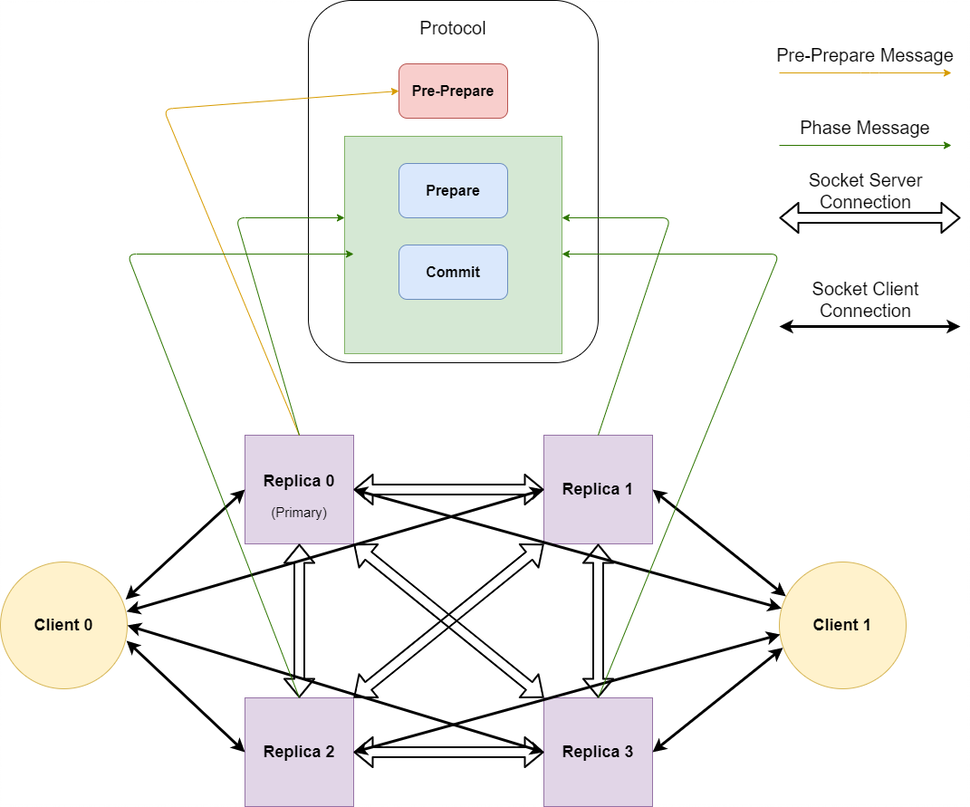
\includegraphics[width=\linewidth]{figures/meshnetwork}
	\caption{Overall architecture of the \ac{pbft} implementation network}
	\label{fig:meshnetwork}
\end{figure}
%NEED TO REDESIGN SO THAT NETWORK IS MENTION IN ONE PART AND OTHER STUFF IN ANOTHER SUBTITLE
The \autoref{fig:meshnetwork} shows the system architecture used for \ac{pbft} implementation. Generally our network architecture follows the same structure as the system model introduced in \autoref{sec:systemModel}. The system consists of four server implementations called \emph{replicas}, where the replica with the lowest identifier value is chosen as the primary. These four replicas are communicating over a mesh network using socket connections. This means each replica shares a unique network socket with each other replica in the \ac{pbft} network. To avoid creating multiple socket connections between two replicas, the replica with the highest identifier is the one tasked with being the initiator when creating the socket connection. Because of this the primary replica is not required to be an active party when establishing any connections to its fellow replicas. The primary instead establishes all its socket connections by listening for any connection attempts on its local network address. The opposite scenario occurs for the replica with the highest identifier value. Although the replica still listens for connections on its local network address in the case where a higher replica does exist in the network, it is also responsible for initiating the socket connections with all the other replicas in the network that have lower identifier values to its own.

When the replicas have established connections, the replicas can still not fully communicate with each other until they have exchanged public keys. This is required so that messages between replicas can be verified using a digital signature. Public keys are exchanged in \emph{session messages}, which are messages that are automatically sent between replicas once a socket connection has been established. If the public keys are for some reason not exchanged, then the replica discards any message received from that host. If the message received from the unknown host happens to be a \emph{request} or a protocol-related message, the replica also terminates the connection. This also applies for clients. This current public key model is unfortunately not very secure. This is due to public keys being ephemeral, therefore it needs to be updated and replaced in the case the replica’s execution is interrupted or stopped. Currently in this implementation, the private and public key pair for a replica are created randomly at system start-up. Currently there is no way for the replicas to authenticate another replica after it has rebooted. A replica must therefore replace the key value pair representing a replica's public key in its register if it receives a new session message with the same replica identifier value. This in turn means the system is susceptible to impersonation and spoofing attacks~\cite{WEB:spoofingAttack}. Because the main goal of this thesis focuses more on the aspects behind implementing a simple \ac{pbft} workflow, the current cryptographic system was deemed sufficient for simulating a network using digital signatures. However, it is important to be aware of this major security flaw of the system so that it can be potentially fixed in the future. Not to mention avoid similar problems in the future.


\section{Overview of Workflow}
The system performs the \ac{pbft} protocol by exchanging protocol messages over the mesh network until at least three of the servers have finished all three protocol phases. In this implementation protocol messages. The \ac{pbft} protocol is triggered when the server receives a request from one of the connected client nodes. The primary is responsible for officially starting an instance of the \ac{pbft} protocol by multicasting a protocol message of type pre-prepare. There are two important goals for the pre-prepare phase. The first is to make sure that the replicas have an agreement upon the ordering of the request. In other words, the replicas will perform the requests in the same order as the primary, which in turn means the request should have the same sequence numbers throughout the network. The second important goal is to determine whether or not the primary is fit to be leader. As mentioned in section \autoref{sec:view-change}, a view-change occurs when a leader no longer is eligible. In our application the view-changes are triggered by timeout which are set once a replica receives a client's request. If the primary takes too long in the pre-prepare phase, then the timeout will exceed and the other replicas will perform a view-change in order to change the primary replica. Although it would be useful to have timeouts in the commit phase in the instance where the majority of servers are unable to properly finish the commit phase, it is currently not supported in our implementation due to how timeouts are handled inside the protocol workflow(should probably be moved elsewhere). The rest of the replicas will be the responsible party during the prepare phase by sending protocol messages of type prepare, while every replica will participate in the commit phase using commit type protocol messages. The last step of current \ac{pbft} implementation is to create a reply message and send it back to the client responsible for the request. The details in regards to the \ac{pbft} workflow implementation will be discussed in \autoref{chapter:Imp}.

\section{Code structure}
In the figure we \autoref{fig:filestruct} can see a short summary of the code structure for our \ac{pbft} replica. The summary shows folders containing our implementation for necessary items for the \ac{pbft}. The summary also highlights some of the more important files, meaning files that contain the most relevant code segments for the application.

%REWRITE SO THAT THE FOCUS IS ON THE Code structure how protocol functionality is %divided into different class objects and divided etc. Then talk about the server.cs <--> %workflow relationship, started by App.cs

\subsection{Protocol Objects}
To start off, the \ac{pbft} algorithm uses a lot of different types of message for the replicas to collaborate. For simplicity we stored all of the classes revolving messages within the \emph{Message} folder. Since the protocol messages share traits and functionality, we introduced two interfaces to reduce redundancy. The first interface regards the serialization process for transforming the messages into byte streams so that they can be exchanged over the \ac{tcp} network~\cite{WEB:tcp}. The other interface is for the digital signature process. Session messages are not signed, therefore they do not inherit this interface. In addition, to reduce complexity we set the normal workflow protocol messages such as pre-prepare, prepare and commit messages, to use a single class object known as \code{Phase Messages}. View-change and checkpoint messages are instead represented with their own unique class object.

To store the proof of an \ac{pbft} iteration, we implemented class objects known as \emph{certificates} that are found in the \emph{Certificates} folder. The implemented certificate objects essentially have the same functionality as the different certificates described in \autoref{chapter:PBFT} for the \ac{pbft} algorithm. Certificates act as records showing the status of the state of protocol iteration, where a single iteration requires 2 valid certificates in order to finish. Just like the protocol messages, we implement both protocol certificate types by an object class known as \code{Protocol certificate} where the protocol types are determined by a single variable. Checkpoints and view-changes once again have their own class object for their certificate proof. There are also interfaces used to avoid redundant code for the certificate objects.

\subsection{Other functionalities}
The static functionalities that are not tied to any object classes are placed in the \emph{Helper} folder. This includes functionality for serializing and deserializing messages objects with \ac{json}~\cite{WEB:NewJSON}, cryptographic functions related to creating and validating digital signatures and files containing all the enum types used for this implementation. An enum is essentially a predefined dotnet class that has only constant values which are defined upon initialization and is really useful for classifying other objects~\cite{WEB:Enum}. In our \ac{pbft} implementation we have for instance used enums to categorize the protocol phase a phase message belongs to. This allows the program to easily distinguish between pre-prepare, prepare and commit phase messages even when they all use the same object type.

The \emph{JSONFiles} folder contains the \ac{json} files which have information about the network addresses for each of the replicas in the system designated to their receptive identifier values. There exist two \ac{json} files in this folder. The first file is used when running the implementation over multiple systems or over docker containers. The second file uses localhost addresses with different port numbers that are meant to be used when testing the system on a local device.

The \ac{pbft} replica implementation uses Cleipnir to persist important parts of the code in order for servers to easily be able to reconnect to the system. As discussed in \autoref{chapter:Cleipnir}, Cleipnir has several different engine types which can be used to serialize and store the applications data. In our \ac{pbft} replica implementation, we have decided to use the \emph{Simple File Storage} engine. The \emph{Storage} folder will contain the .txt files in which Cleipnir stores its data in. Since there are several instances of replicas in the \ac{pbft} network, the name of the .txt file used to store the application data will follow the structure "PBFTStorage" with the replicas identifier value at the end of the name.

The \emph{Replica} folder contains code which is directly related to the server or code which are directly related to the protocol. The \emph{Replica} folder has two sub folders in order to easier distinguish code based on their functionality. All the networking code that is not directly connected to the server side network handling is placed inside the subfolder \emph{Network}. This includes the code for creating sockets and functions for properly handling the data received from the socket by the TCP network protocol.
The \emph{Protocol} sub folder contains code which is directly related to the protocol execution. This includes code related to the execution of the main workflow of the \ac{pbft} algorithm. In addition, code for handling the reactive execution for view-change and checkpointing are also placed here.
The other files in the \emph{Replica} folder contains code that helps the replica run properly, including code which is used to help communication between server side and protocol workflow run inside Cleipnir.

\subsection{JSON Serialization Problem}
As mentioned in \autoref{section:PersistentProgramming} Cleipnir requires a designated serializer and deserializer function in order to persist an object. In addition, Cleipnir cannot persist traditional data structures directly. Instead Cleipnir intends for the developer to substitute traditional data structures with Cleipnir respective inbuilt data structures. This means that whenever Cleipnir persists objects that have a reference to a data structure, then the persisted object must also substitute the data structure for correct inbuilt Cleipnir data structure. For our case this is present for all of our \code{Certificate} objects as they all require a list of proofs. Therefore in order to persist the proof list, we need to replace a traditional \code{List} class object with an inbuilt \code{CList} class object. However, Cleipnir inbuilt data structures cannot be serialized or deserialized properly using \ac{json} formatting. As we were not completely aware of this issue when we began designing our application, we unfortunately made an oversight for our network layer. The application currently uses \ac{json}~\cite{WEB:NewJSON} to serialize and deserialize messages when sent over the \ac{pbft} network. Since \ac{json} formatting does not support inbuilt Cleipnir data structures, which in retrospect was not all that surprising, attempting to deserialize any protocol message that includes an inbuilt Cleipnir data structure, causes the application to crash. Currently we solve this issue by converting between traditional data structures and inbuilt Cleipnir data structures whenever a message with said data structure is to be serialized with \ac{json}. The conversion itself is rather primitive. A copy of the data storage in the traditional data structure format is created, then the content is copied from the source data storage to the newly created data storage. The process is then reversed on the receiver end after the message has been properly deserialized. To further simplify the conversion between the data structure types, we added temporary \code{\ac{json}} class objects that acts as substitutes for the persisted objects that have issues with \ac{json} when they are to be sent over the \ac{pbft} network. Transforming between a persisted object to their respective temporary \ac{json} object is as simple as making a function call with the opposite transformation also available. These \ac{json} objects are all placed in the subfolder \code{JsonObjects} in the \code{Helper} folder. All implemented \ac{json} class objects follow the naming convention $JSON + Objectname$. Having now learned about this issue it properly would have been more beneficial if the serialization and deserialization for the networking used the same formatting in which Cleipnir supports, as to avoid this issue in the future projects.

%In order for this to be done the persistable objects needed to be assigned a serializer function and deserializer function for Cleipnir to use. This also includes using Cleipnir inbuilt data structures when the persisted objects needed to also persist data stored in data structures. This is especially present in certificates since they need to persist their list of proofs, meaning the proof list uses the inbuilt Cleipnir \code{CList} to substitute normal List class objects. Unfortunately we made an oversight when we designed the application. The application currently uses \ac{json}~\cite{WEB:NewJSON} to serialize and deserialize messages when sent over the \ac{pbft} network. \ac{json} formatting does not support inbuilt Cleipnir data structures, which is not surprising yet was not directly discovered until very late into the \ac{pbft} implementation. Currently this issue is solved by converting between traditional data structures and inbuilt Cleipnir data structures whenever a message with said data structure is to be serialized by \ac{json}. The conversion itself is rather primitive. A copy of the data storage in the traditional data structure format is created, then the content is copied from the source data storage to the newly created data storage. The process is then reversed on the receiver end after the message has been properly deserialized. Although in retrospect, it might have been more beneficial if the serialization and deserialization for the networking used the same format in which Cleipnir supports, as to avoid this issue in the future

\subsection{Notable Files}
The \emph{App.cs} file contains the code which starts all the processes needed in the \ac{pbft} replica. This includes code for starting Cleipnir, creating a server instance and starting the protocol handlers. This file also includes the main application state, which in this implementation is simply a list of operations theoretically performed by the system.

The \emph{Server.cs} file is by far the largest. This is due to the server this implementation  acts as the bridge linking the network layer, responsible for sending and receiving messages properly, to the active protocol workflow which requires the result of said messages. In general the server is also responsible for the other server side operations.

The \emph{Workflow.cs} file is where the code for normal protocol workflow and view-change workflow occurs. The \autoref{chapter:Imp} introduces in detail how the workflows are implemented.
%\newpage
\begin{wrapfigure}{r}{0.45\linewidth}
\centering
%\vspace{15pt}
%\rule{0.9\linewidth}{0.75\linewidth}
% ,scale=0.8, every node/.style={scale=0.8}
\tikzstyle{every node}=[draw=black,thick,anchor=west]
    \begin{tikzpicture}[%
      grow via three points={one child at (0.5,-0.7) and
      two children at (0.5,-0.7) and (0.5,-1.4)},
      edge from parent path={(\tikzparentnode.south) |- (\tikzchildnode.west)}]
      \node {PBFT}
        child { node {App.cs}}
        child { node {Certificates}
        	child {node {...}}
        	}	
        child [missing] {}
        child { node {Messages}
        	child {node {...}}
        	}
        child [missing] {}
        child { node {Helper}
        	child {node {...}}
        	}
        child [missing] {}
        child { node {JSONFiles}
        	child {node {serverInfo.json}}
        	child {node {testServerInfo.json}}
        	}
        child [missing] {}
        child [missing] {}
        child { node {Storage}
        	child {node {...}}
        }
        child [missing] {}
        child { node {Replica}
          child { node {Server.cs}}
          child { node {Network}
          	child {node {...}}
        	}
        }
        child [missing] {
          child { node {Protocol}
          child { node {Workflow.cs}}
          child { node {...}}
        	}
        };
\end{tikzpicture}
    \caption{Summary of the file architecture for the PBFT implementation}
    \label{fig:filestruct}
    \vspace{40pt}
\end{wrapfigure}
\fi

This chapter presents an overall summary of our \ac{pbft} application implementation. This includes a description of the system architecture used for the \ac{pbft} network. Additionally, to better understand the application’s workflow, a summary of our code structure is given. Finally, a description is provided for the current application design. Primarily specifying which parts of the program take advantage of the Cleipnir framework and how the server-side interacts with the protocol workflow.
%Remember to check previous sections for how I should mark names in the text!
\section{Network Architecture}
\begin{figure}
	\centering
	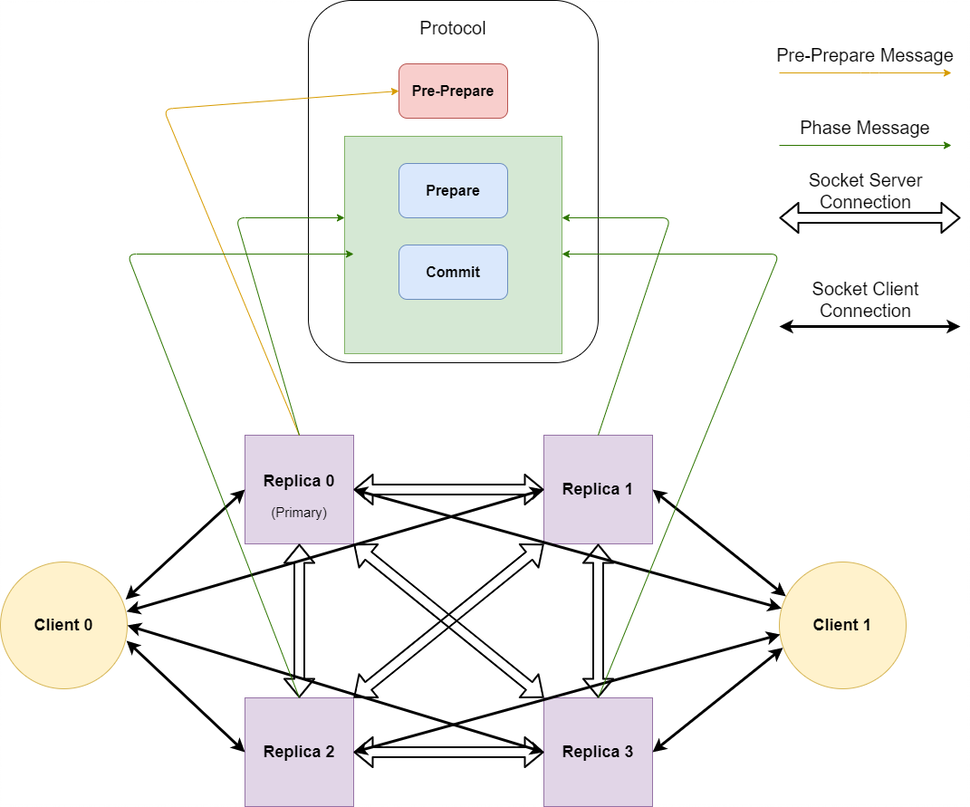
\includegraphics[width=\linewidth]{figures/meshnetwork}
	\caption{Overall architecture of the \ac{pbft} implementation network}
	\label{fig:meshnetwork}
\end{figure}
\autoref{fig:meshnetwork} shows the system architecture used for \ac{pbft} implementation. Generally, our network architecture follows the same structure as the system model introduced in \autoref{sec:systemModel}. The system consists of four server implementations called \emph{replicas}, where the replica with the lowest identifier value is chosen as the primary. These four replicas are communicating over a mesh network using socket connections. This means that each replica shares a unique network socket with each of the other replicas in the \ac{pbft} network. To avoid creating multiple socket connections between two replicas, the replica with the highest identifier is tasked with being the initiator when creating the socket connection. Because of this, the primary replica is not required to actively establish any of its connections to its fellow replicas. Instead, the primary establishes all its socket connections by listening for any connection attempts on its local network address. The opposite scenario occurs for the replica with the highest identifier value. Although the other non-primary replicas also listen for connections on their local network address, this is done to connect to replicas with higher ids in the network. The non-primary replica is also responsible for initiating the socket connections with all the other replicas in the network with lower identifier values.

When the replicas have established connections, the replicas can still not fully communicate until they have exchanged public keys. This is required so that messages between replicas can be verified using a digital signature. Public keys are exchanged in \emph{session messages}, which are messages that are automatically sent between replicas once a socket connection has been established. If the public keys are for some reason not exchanged, then the replica discards any message received from that host. If the message received from the unknown host happens to be a \emph{request} or a protocol-related message, the replica also terminates the connection. This also applies to clients. This current public key model is unfortunately not very secure. This is due to public keys being ephemeral. Therefore, it needs to be updated and replaced if the replica’s execution is interrupted or stopped.
In this implementation, the private and public key pair for a replica is created at the system start-up. Currently, there is no way for the replicas to authenticate another replica after it has rebooted. Therefore, a replica must replace the key-value pair representing a replica’s public key in its register if it receives a new session message with the equal replica identifier value. This, in turn, means the system is susceptible to impersonation and spoofing attacks~\cite{WEB:spoofingAttack}. Because the main goal of this thesis focuses more on the aspects behind implementing a simple \ac{pbft} workflow, the current cryptographic system was deemed sufficient for simulating a network using digital signatures. However, it is important to be aware of this major security flaw of the system to be potentially fixed and avoided in the future.

\section{Overview of Workflow}
The system performs the \ac{pbft} protocol by exchanging protocol messages over the mesh network until at least three replica implementations have finished all three protocol phases. The \ac{pbft} protocol is triggered when the server receives a request from one of the connected client nodes. The primary is responsible for officially starting an instance of the \ac{pbft} protocol by multicasting a protocol message of type pre-prepare. There are two important goals for the pre-prepare phase. The first is to make sure that the replicas have an agreement upon the ordering of the request. In other words, the replicas perform the requests in the same order as the primary, which means a request processed over several replicas should all be using the same sequence number for processing that request. The second important goal is to determine whether or not the primary is fit to be the leader. As mentioned in section \autoref{sec:view-change}, a view-change occurs when a leader no longer is eligible. The view-changes are triggered by timeout functionality in our application, which is set once a replica receives a client request. If the primary takes too long in the pre-prepare phase, then the timeout occurs, and the other replicas perform a view-change to change the primary replica. 
The rest of the replicas are the responsible parties during the prepare phase by sending protocol messages of type prepare, while every replica participates in the commit phase using commit type protocol messages. The last step of the current \ac{pbft} implementation is to create a reply message and send it back to the client responsible for the request. The details in regards to the \ac{pbft} workflow implementation is discussed in \autoref{chapter:Imp}.
%Although it would be useful to have timeouts in the commit phase where the majority of replicas cannot finish the commit phase properly, it is currently not supported in our implementation due to how timeouts are handled inside the protocol workflow. (should probably be moved elsewhere). 

\section{Code structure}
In \autoref{fig:filestruct} shows a figure that illustrates a short summary of the code structure used for our \ac{pbft} replica implementation. The summary shows folders containing our source code used to implement the necessary items for the \ac{pbft} algorithm. The summary also highlights some of the more important files, meaning files that contain the most relevant code segments for the application.

%REWRITE SO THAT THE FOCUS IS ON THE Code structure how protocol functionality is %divided into different class objects and divided etc. Then talk about the server.cs <--> %workflow relationship, started by App.cs

\subsection{Protocol Objects}
To start off, the \ac{pbft} algorithm uses many different types of messages for the replicas to collaborate. For simplicity, we stored all of the classes revolving messages within the \emph{Message} folder. Since the protocol messages share traits and functionality, we introduced two interfaces to reduce redundancy. The first interface regards the serialization process for transforming the messages into byte streams so that to allow the message objects to be exchanged over the \ac{tcp} ~\cite{WEB:tcp}. The other interface is for the digital signature process. Session messages are not signed; therefore, they do not inherit this interface. In addition, to reduce complexity, we set the normal workflow protocol messages such as pre-prepare, prepare and commit messages, to use a single class object known as \code{Phase Messages}. A single value within the \code{Phase Message} object designates which protocol type the \code{Phase Message} represents. View-change and checkpoint messages are instead represented with their own unique class object.

To store the proof of an \ac{pbft} iteration, we implemented class objects known as \emph{certificates} found in the \emph{Certificates} folder. The implemented certificate objects essentially have the same functionality as the different certificates described in \autoref{chapter:PBFT} for the \ac{pbft} algorithm. Certificates act as records showing the state of protocol iteration, where a single iteration requires two valid certificates before the iteration is deemed finished. Just like the protocol messages, we implement both protocol certificate types by an object class known as \code{Protocol certificate} where a single variable determines the protocol types. Checkpoints and view-changes once again have their own class object for their certificate proof. There are also interfaces used to avoid redundant code for the certificate objects. The interfaces used for certificates are primarily used to add the mandatory functions for a given certificate object. 

\subsection{Other functionalities}
The static functionalities that are not tied to any object classes are placed in the \emph{Helper} folder. This includes functionality for serializing and deserializing messages objects with \ac{json}~\cite{WEB:NewJSON}, cryptographic functions related to creating and validating digital signatures, and files containing all the enum types used for this implementation. An enum is essentially a predefined .NET class with only constant values. The enum’s constant values are defined upon initialization and are helpful for classifying other objects~\cite{WEB:Enum}. For instance, our \ac{pbft} implementation has used enums to categorize the protocol phase a phase message belongs to. This allows the program to easily distinguish between pre-prepare, prepare and commit phase messages even when they all use the same object type.

The \emph{JSONFiles} folder contains the \ac{json} files, which have information about the network addresses for the replicas in the system designated to their receptive identifier values. There exist two \ac{json} files in this folder. The first file is used when running the implementation over multiple systems or over docker containers. The second file uses localhost addresses with different port numbers that are meant to be used when testing the application on a local device.

The \ac{pbft} replica implementation uses Cleipnir to persist important parts of the code for servers to be able to reconnect to the system easily. As discussed in \autoref{chapter:Cleipnir}, Cleipnir has several different engine types, which can be used to serialize and store the application’s data. In our \ac{pbft} replica implementation, we have decided to use the \emph{Simple File Storage} engine. The \emph{Storage} folder will contain the .txt files in which Cleipnir stores its data. Since there are several instances of replicas in the \ac{pbft} network, the name of the .txt file used to store the application data will follow the structure “PBFTStorage” with the replicas identifier value at the end of the name.

The \emph{Replica} folder contains code that is directly related to the server or the protocol workflow. The \emph{Replica} folder has two subfolders in order to distinguish code based on their functionality easier. All the networking code that is not directly connected to the server-side network handling is placed inside the subfolder \emph{Network}. This includes the code for creating sockets and functions for properly handling the data received from the socket by the TCP network protocol.
The \emph{Protocol} subfolder contains code that is directly related to the protocol execution. This includes code related to the execution of the main workflow of the \ac{pbft} algorithm. In addition, code for handling the reactive execution for view-change and checkpointing is also placed here.
The other files in the \emph{Replica} folder contain code that helps the replica run properly, including code used to help communication between server-side and protocol workflow run inside Cleipnir.

\subsection{JSON Serialization Problem}
As mentioned in \autoref{section:PersistentProgramming} Cleipnir requires a designated serializer and deserializer function to persist an object. In addition, Cleipnir cannot persist traditional data structures directly. Instead, Cleipnir intends for the developer to substitute traditional data structures with Cleipnir respective inbuilt data structures. This means that whenever Cleipnir persists objects that have a reference to a data structure, then the persisted object must also substitute the data structure for the correct inbuilt Cleipnir data structure. For our implementation, this is present in our \code{Certificate} objects as they all require a list of proofs. Therefore to persist the proof list, we need to replace a traditional \code{List} class object with an inbuilt \code{CList} class object. However, Cleipnir inbuilt data structures cannot be serialized or deserialized properly using \ac{json} formatting.
As we were not completely aware of this issue when we began designing our application, we, unfortunately, made an oversight for our network layer. The application currently uses \ac{json}~\cite{WEB:NewJSON} to serialize and deserialize messages when sent over the \ac{pbft} network. Since \ac{json} formatting does not support inbuilt Cleipnir data structures, which in retrospect was not all that surprising, attempting to deserialize any protocol message that includes an inbuilt Cleipnir data structure, causes the application to crash. Currently, we solve this issue by converting between traditional data structures and inbuilt Cleipnir data structures whenever a message with said data structure is to be serialized with \ac{json}. The conversion itself is rather primitive. A copy of the data storage in the traditional data structure format is created, then the content is copied from the source data storage to the newly created data storage. The process is then reversed on the receiver end after the message has been properly deserialized. To further simplify the conversion between the data structure types, we added temporary \code{\ac{json}} class objects that act as substitutes for the persisted objects that have issues with \ac{json} when they are to be sent over the \ac{pbft} network. Transforming between a persisted object to their respective temporary \ac{json} object is as simple as making a function call with the opposite transformation also available as a function tied to the temporary object. These \ac{json} objects are all placed in the subfolder \code{JsonObjects} inside the \code{Helper} folder. All implemented \ac{json} class objects follow the naming convention $JSON + Objectname$. Having now learned about this issue, it would have probably been more beneficial if the serialization and deserialization for the networking used the same formatting that Cleipnir supports to avoid this issue in future projects.

\subsection{Notable Files}
The \emph{App.cs} file contains the code which starts all the processes needed in the \ac{pbft} replica. This includes code for starting Cleipnir, creating a server instance, and starting the protocol handlers. This file also includes the main application state, which in this implementation is simply a list of operations theoretically performed by the system.

The \emph{Server.cs} file is by far the largest, and this is due to the server implementation acts as the bridge between the network layer and the protocol workflow. This is necessary as the network layer is responsible for formatting protocol messages being sent to and received from the \ac{pbft} network. On the other hand, the protocol workflows require the protocol messages to finish all of their jobs. The protocol workflows receive the messages from the network layer by having the server implementation schedule emits to the respective workflows \code{Source} object.  The server is also responsible for the other server-side operations.

The \emph{Workflow.cs} file is where the code for normal protocol workflow and view-change workflow occurs. \autoref{chapter:Imp} introduces in detail how the workflows are implemented.
%\newpage
\begin{wrapfigure}{r}{0.45\linewidth}
\centering
%\vspace{15pt}
%\rule{0.9\linewidth}{0.75\linewidth}
% ,scale=0.8, every node/.style={scale=0.8}
\tikzstyle{every node}=[draw=black,thick,anchor=west]
    \begin{tikzpicture}[%
      grow via three points={one child at (0.5,-0.7) and
      two children at (0.5,-0.7) and (0.5,-1.4)},
      edge from parent path={(\tikzparentnode.south) |- (\tikzchildnode.west)}]
      \node {PBFT}
        child { node {App.cs}}
        child { node {Certificates}
        	child {node {...}}
        	}	
        child [missing] {}
        child { node {Messages}
        	child {node {...}}
        	}
        child [missing] {}
        child { node {Helper}
        	child {node {...}}
        	}
        child [missing] {}
        child { node {JSONFiles}
        	child {node {serverInfo.json}}
        	child {node {testServerInfo.json}}
        	}
        child [missing] {}
        child [missing] {}
        child { node {Storage}
        	child {node {...}}
        }
        child [missing] {}
        child { node {Replica}
          child { node {Server.cs}}
          child { node {Network}
          	child {node {...}}
        	}
        }
        child [missing] {
          child { node {Protocol}
          child { node {Workflow.cs}}
          child { node {...}}
        	}
        };
\end{tikzpicture}
    \caption{Summary of the file architecture for the PBFT implementation}
    \label{fig:filestruct}
    \vspace{40pt}
\end{wrapfigure}

\begin{figure}[H]
	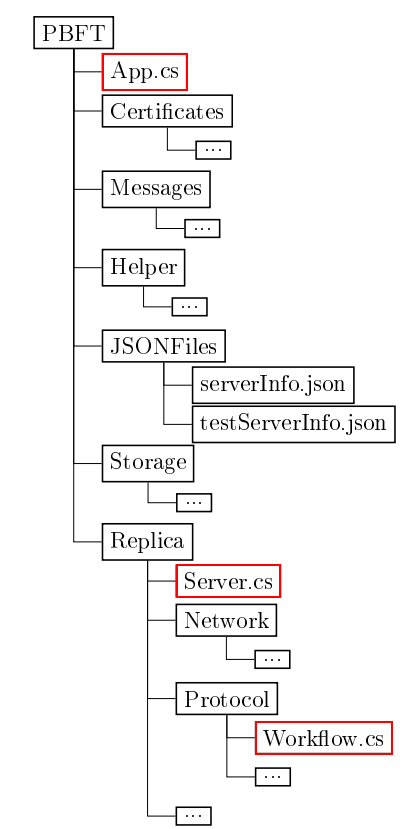
\includegraphics[width=0.45\linewidth]{figures/filestructtest}
	\caption{Summary of the file architecture for the \ac{pbft} implementation}
    \label{fig:filestruct}
\end{figure}

\newpage

\section{Persistent vs Ephemeral}
%This will be a very large part, just need to figure out how to structure it.
%Before we can introduce the main PBFT implementation workflow, it is first important to introduce the relationship between the server side and the protocol workflow.
%\label{sec:persvsephe}
%An important detail when using the Cleipnir framework is to have a general idea for which parts of the system are desired to be persistent. As mentioned in \autoref{section:PersistentProgramming}, Cleipnir allows for hybrid persistent programming allowing the developer the freedom to choose which parts of the application to persist while keeping the rest of the data ephemeral. In our case it was important to figure out which data needed to be persisted in order for the \ac{pbft} algorithm to be easily reinstated should the system shutdown. In addition, when taking advantage of hybrid persistent programming it is important to avoid storing a lot of unnecessary data as it generally slows down the synchronization period. Another reason as to why making a distinct divide between persistent and ephemeral parts of the code is important is due to the difficulties encountered when using \code{CTask} together with traditional asynchronous operations as mentioned in \autoref{section:PersistentProgramming}. In our case, because our goal is to evaluate both async/await and Cleipnir for implementation of consensus algorithms, it is important to not interchange these tools as it would in most cases lead to race conditions.

%\autoref{fig:PersistencyEphemeral} we show parts of our \ac{pbft} implementation that are divided into persistent parts and ephemeral parts. In addition the figure shows an illustration as to how ephemeral parts and the persistent parts collaborate using arrows to dictate the program flow. In general for our application, static functions and objects unrelated to the \ac{pbft} workflow are treated as ephemeral. Meanwhile objects related to the \ac{pbft} implementations, \code{Source} objects and functions that handle workflow related to the \ac{pbft} protocol are persisted. The server is an exception as some parts are persistent while others parts are not. As an example, the protocol logger is stored in the server and is persisted, on the other hand any code related to networking in the server is not persisted. In a sense we can view some of the operations occurring in the server as being treated as a bridge between the persistent parts as well as the ephemeral parts. By this we mean that the server is responsible for handling any messages received from the ephemeral socket connections and delivering them to the appropriate protocol workflow that is persistent. 

%These messages are then emitted to their respective reactive operators which are run in the persistent part and are waiting for changes to occur. There are a few exceptions to this rule, case in point if the message is needed for server-side rather than any \ac{pbft} protocol workflows, the message is instead used directly by the server. A primary example of this being session messages. However, in order for the server's non-persistent network handler to perform operations which affect the persistent part run by Cleipnir, the operation must be scheduled by Cleipnir's execution engine. There are two reasons for this syntax. 

%Firstly, code run by Cleipnir is not supposed to be affected by code outside of Cleipnir. Similarly to the case where using asynchronous operations within \code{CTask}, attempting to emit a message or perform an operation which changes the state of a persisted object, will most of the time cause the same scenario we discussed earlier in \autoref{chapter:Cleipnir}. New threads are created and Cleipnir attempts to perform the operation concurrently, however this scenario is not thread safe and sooner or later causes issues for the state of the system negatively. 
%\ac{fcfs}
%Secondly, running operations though the Cleipnir's execution engine attempts to enforce the operations to be run in a \ac{fcfs} approach as mentioned in \autoref{section:CleipnirOv}. This will in turn make it a lot easier to keep track of the operations as it gives the illusion of a synchronous system. The only situation we experienced where the Cleipnir execution engine didn't follow the \ac{fcfs} scheduling algorithm was when the next operation was stuck, in which the second operation in the queue line was executed instead and so forth. \autoref{code:schedulerEmit} shows an example of where the server uses the Cleipnir engine reference to schedule a phase message to be emitted to the \emph{ProtocolSubject} \code{Source} object. To summarize the primary relationship between the server, the network layer and the persistent workflow implementations is simply that the server will emit any messages it receives from the network layer and then emit these messages to the persistent workflows. As it is required for the \ac{pbft} protocol and view-change protocol to multicast messages during their process, these implementations have a direct reference to the server. In order to accomplish this, both persistent workflow shares a common persistent object known as \code{ProtocolExecution}. This means the protocol algorithms can easily send any messages it needs to the server through the server referance in the \code{ProtocolExecution}. REWRITE NOWWWWW

%This design is unfortunately not perfect. Because the server is required to schedule the operations in order for protocol execution to move on with its execution. We have encountered some situations where the scheduled process never finishes its execution. This wouldn’t be considered a big issue most of the time as the application is run asynchronously, however there are some instances where this situation can become a big problem.. Usually when scheduling an operation which requires emitting an object to a \code{Source} object that currently does not have any receivers, the operation obviously never finishes. When the server attempts to schedule an additional operation afterwards, the operation is never scheduled, which in turn leads to the application being deadlocked. This situation seems to be similar to sending messages to a channel without any receivers in Golang~\cite{WEB:golangChannels}, in spite of that this is an issue which rarely occurs, but when it does it is detrimental to the system. Therefore, to counteract this issue, strict conditions are placed in the server to avoid sending messages to reactive subjects in the situations where there are no listeners.

\iffalse
\label{sec:persvsephe}
An important detail when using the Cleipnir framework is to have a general idea for which parts of the system are desired to be persistent. As mentioned in \autoref{section:PersistentProgramming}, Cleipnir allows for hybrid persistent programming allowing the developer the freedom to choose which parts of the application to persist while keeping the rest of the data ephemeral. In our case it was important to figure out which data is needed to be persisted in order for the \ac{pbft} algorithm to be easily reinstated should the system shutdown. In addition, when taking advantage of hybrid persistent programming it is important to avoid storing a lot of unnecessary data as it generally slows down the synchronization period. Another reason as to why making a distinct divide between persistent and ephemeral parts of the code is important is due to the difficulties encountered when using \code{CTask} together with traditional asynchronous operations as mentioned in \autoref{section:PersistentProgramming}. In our case, because our goal is to evaluate both async/await and Cleipnir for implementation of consensus algorithms, it is important to not interchange these tools as it would in most cases lead to race conditions.

\autoref{fig:PersistencyEphemeral} we show parts of our \ac{pbft} implementation that are divided into persistent parts and ephemeral parts. In addition the figure shows an illustration as to how ephemeral parts and the persistent parts collaborate using arrows to dictate the program flow. In general for our application, static functions and objects unrelated to the \ac{pbft} workflow are treated as ephemeral. Meanwhile objects related to the \ac{pbft} implementations, \code{Source} objects and functions that handle workflow related to the \ac{pbft} protocol are persisted. The server is an exception as some parts are persistent while others parts are not. As an example, the protocol logger is stored in the server and is persisted, on the other hand any code related to networking in the server is not persisted. In a sense we can view some of the operations occurring in the server as being treated as a bridge between the persistent parts as well as the ephemeral parts. By this we mean that the server is responsible for handling any messages received from the ephemeral socket connections and delivering them to the appropriate protocol workflow that is persistent. 

These messages are then emitted to their respective reactive operators which are run in the persistent part and are waiting for changes to occur. There are a few exceptions to this rule, case in point if the message is needed for server-side rather than any \ac{pbft} protocol workflows, the message is instead used directly by the server. A primary example of this being session messages. However, in order for the server's non-persistent network handler to perform operations which affect the persistent part run by Cleipnir, the operation must be scheduled by Cleipnir's execution engine. There are two reasons for this syntax. 

Firstly, code run by Cleipnir is not supposed to be affected by code outside of Cleipnir. However, since the protocol workflow relies on messages from the non-persistent network layer this cannot be avoided in our application. Therefore a way for the persistent and non-persistent areas to work together must be coordinated. To start, attempting to emit a message to a \code{Source} object or perform an operation which changes the state of a persisted object outside of a \code{CTask} function, can cause the same scenario we discussed earlier in \autoref{chapter:Cleipnir}. That is, new threads are created and Cleipnir attempts to perform the operation concurrently, however this scenario is not always thread safe and sooner or later causes issues for the state of the system negatively. 

It is intended to avoid this problem by using the Cleipnir execution engine directly to schedule the desired operation to be run with Cleipnir support. The Cleipnir execution engine runs its scheduled operations using a \ac{fcfs} approach as mentioned in \autoref{section:CleipnirOv}. Scheduling operations desired for the protocol using the execution engine makes it easier to keep track of operations as they must likely run in a synchronous order with the other operations happening in the protocol workflow. This however this not mean the system is synchronous as Cleipnir only gives an illusion of a synchronous system. The execution engine can change the order of execution while another scheduled operation is idle or stuck.In which case the next scheduled operation is run next. \autoref{code:schedulerEmit} shows an example of how to schedule an operation to the Cleipnir execution engine. In this example where the server schedules a phase message to be emitted to the \code{ProtocolSource} \code{Source} object.

To summarize the relationship between the server, network layer and the persistent protocol workflows is that the server is responsible for emitting any relevant messages received from the network layer to the protocol workflow. In addition, the server is also responsible for preparing and sending any protocol messages it gets from the protocol workflow to the network layer so that the protocol messages are correctly sent to the other replicas in the network. In order for the protocol workflows as an object reference to the server, meaning the protocol workflow calls the appropriate send function in the server object whenever a protocol needs for a protocol message to be sent over the network. Since both the normal protocol workflow and view-change workflow requires multicasting protocol messages to move on in their respective workflows, it is necessary for the workflows to have a direct reference to the server. All protocol workflow that requires the server referanse are all apart of the class known as \code{Workflow} 

This design is unfortunately not perfect. The server is required to schedule the operations in order for the protocol execution to move on with its execution. We have encountered some situations where the scheduled operations to the Cleipnir execution engine never finishes its execution. This wouldn’t be considered a big issue most of the time as the application is run asynchronously, however there are some instances where this situation can become a big problem. Usually when scheduling an operation that requires emitting an item to a \code{Source} object that currently does not have any receivers, the operation obviously never finishes. When the server attempts to schedule an additional operation afterwards, the operation is never scheduled, which in turn leads to the application being deadlocked. This situation seems to be similar to sending messages to a channel without any receivers in Golang~\cite{WEB:golangChannels}, in spite of that this is an issue which rarely occurs, but when it does it is detrimental to the system. Therefore, to counteract this issue, strict conditions are placed in the server to avoid sending messages to reactive subjects in the situations where there are no listeners.
\fi

\label{sec:persvsephe}
An important detail when using the Cleipnir framework is to have a general idea for which parts of the system are desired to be persistent. As mentioned in \autoref{section:PersistentProgramming}, Cleipnir allows for hybrid persistent programming allowing the developer the freedom to choose which parts of the application to persist while keeping the rest of the data ephemeral. In our case, it was essential to figure out which data is needed to be persisted for the \ac{pbft} algorithm to be easily reinstated should the system shutdown. In addition, when taking advantage of hybrid persistent programming, it is important to avoid storing a lot of unnecessary data as it generally slows down the synchronization period. Another reason why making a distinct divide between persistent and ephemeral parts of the code is important is due to the difficulties encountered when using \code{CTask} together with traditional asynchronous operations, as mentioned in \autoref{section:PersistentProgramming}. In our case, because our goal is to evaluate both async/await and Cleipnir for implementation of consensus algorithms, it is crucial to not interchange these tools as it would, in most cases, lead to race conditions.

\autoref{fig:PersistencyEphemeral} shows parts of our \ac{pbft} implementation that are divided into persistent parts and ephemeral parts. In addition, the figure shows an illustration of how ephemeral parts and persistent parts collaborate using arrows to dictate the program flow. In general, for our application, static functions and objects unrelated to the \ac{pbft} workflow are treated as ephemeral. Meanwhile, objects related to the \ac{pbft} implementations, \code{Source} objects and functions that handle workflow related to the \ac{pbft} protocol are persisted. The server is an exception as some parts are persistent while others parts are not. For example, the protocol logger is stored in the server and is persisted; on the other hand, any code related to networking in the server is not persisted.  We can view certain operations occurring in the server as being treated as a bridge between the persistent part and the ephemeral parts. By this, we mean that the server is responsible for handling any messages received from the ephemeral socket connections and delivering them to the appropriate protocol workflow that is persistent. 

These messages are then emitted to their respective reactive operators, which are run in the persistent part and are waiting for changes to occur. There are a couple of exceptions to this rule. For instance, if the message received is needed for the server-side, the message is used directly by the server. A primary example of this being session messages. However, for the server’s non-persistent network handler to perform operations that affect the persistent part run by Cleipnir, the operation must be scheduled by Cleipnir’s execution engine. There are two reasons for this syntax. 

Firstly, code run by Cleipnir is not supposed to be affected by code outside of Cleipnir. However, since the protocol workflow relies on messages from the non-persistent network layer, our application cannot avoid it. Therefore, a way for the persistent and non-persistent areas to work together must be coordinated. To start, attempting to emit a message to a \code{Source} object or perform an operation that changes the state of a persisted object outside of a \code{CTask} function can cause the same scenario discussed earlier in \autoref{chapter:Cleipnir}. That is, new threads are created, and Cleipnir attempts to perform the operation concurrently. However, this scenario is not always thread-safe and sooner or later causes issues for the system state. 

It is intended to avoid this problem by using the Cleipnir execution engine directly to schedule the desired operation to be run with Cleipnir support. The Cleipnir execution engine runs its scheduled operations using a \ac{fcfs} approach, as mentioned in \autoref{section:CleipnirOv}. Scheduling operations desired for the protocol using the execution engine makes it easier to keep track of operations, as they most likely run in a synchronous order with the other operations happening in the protocol workflow. However, this does not mean the system is synchronous, as Cleipnir only gives an illusion of a synchronous system. The execution engine can change the order of execution while another scheduled operation is idle or stuck. In which case, the next scheduled operation is run. \autoref{code:schedulerEmit} shows an example of how to schedule an operation to the Cleipnir execution engine. In this example, the server schedules a \code{Phase message} to be emitted to the \code{ProtocolSource} \code{Source} object.

To summarize, the relationship between the server, network layer, and the persistent protocol workflows is that the server is responsible for emitting any relevant messages received from the network layer to the protocol workflow. In addition, the server is also responsible for preparing and sending any protocol messages it gets from the protocol workflow to the network layer so that the protocol messages are correctly sent to the other replicas in the network. To accomplish this functionality, the protocol workflows have an object reference to the server. This means the protocol workflow calls the appropriate send function in the server object whenever a protocol workflow needs a protocol message to be sent over the network. Since both the normal protocol workflow and view-change workflow are required to multicast protocol messages to move on in their respective workflows, the workflows must directly reference the server object’s multicast function. All protocol workflows that require the server reference are all a part of the class known as \code{Workflow} 

This design is unfortunately not perfect. Ultimately, since the server is responsible for scheduling the operations revolving around protocol messages, the protocol workflows can become stuck if something happens to the scheduled emit. We have encountered some situations where the scheduled operations to the Cleipnir execution engine never finishes its execution. This would not be considered a big issue most of the time as the application is run asynchronously. However, there are some instances where this situation can become a big problem. Usually, when scheduling an operation that requires emitting an item to a \code{Source} object that currently does not have any receivers, the operation never finishes. When the server attempts to schedule an additional operation afterwards, the operation is never scheduled, leading to the application getting stuck. This situation seems to be similar to sending messages to a channel without any receivers in Golang~\cite{WEB:golangChannels}, despite that this is an issue that rarely occurs, but when it does, it is detrimental to the system. Therefore, to counteract this issue, strict conditions are placed in the server to avoid sending messages to reactive subjects in situations where there are no listeners.

\begin{figure}[H]
	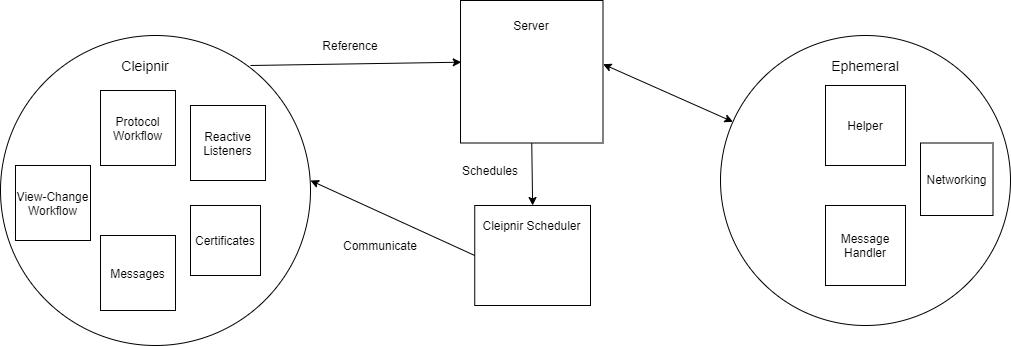
\includegraphics[width=\linewidth]{figures/CleipnirStructure}
	\caption{Application divided into persistent parts and ephermeral parts and how they interact}
	\label{fig:PersistencyEphemeral}
\end{figure}

\begin{figure}[h]
	\centering
	%\lstset{style=sharpc}
	\begin{lstlisting}[label = code:schedulerEmit, caption= Example of server and protocol interaction using Cleipnir scheduler, captionpos=b, basicstyle=\scriptsize]
public void EmitPhaseMessageLocally(PhaseMessage mes)
{
    Console.WriteLine("Emitting Phase Locally!");
    if (ProtocolActive)
    {
        _scheduler.Schedule(() =>
        {
            Subjects.ProtocolSubject.Emit(mes);
        });   
    }
}
	\end{lstlisting}
\end{figure}
